\section{Problemas NP-Completo}
Problemas NP-Completo são problemas que são NP e também é tão "difícil" quanto todos os outros problemas NP, e isso deve ser provado matematicamente assim como o \textit{Teorema de Cook} com o \textit{Problema SAT}, uma vez que não é possível prová-los um-a-um devido a grande quantidade de problemas NP.

	\begin{figure}[H]
		\centering
		\label{fig1}
		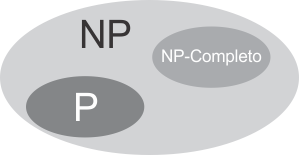
\includegraphics[scale=2]{./figuras/figProblemas.png}
		\caption{O modo como grande parte dos cientistas da computação vê os relacinamentos entre P, NP e NPC. Tanto P quanto NPC estão completamente contidas dentro de NP, e $P \cap NP-Completo = \phi$ \cite{leisersonalgoritmos}}
	\end{figure}

